% Source: https://tex.stackexchange.com/a/642555/6880

\documentclass[border=3.141592]{standalone}
\usepackage{tikz}
\usetikzlibrary{calc,
                positioning}

\begin{document}
    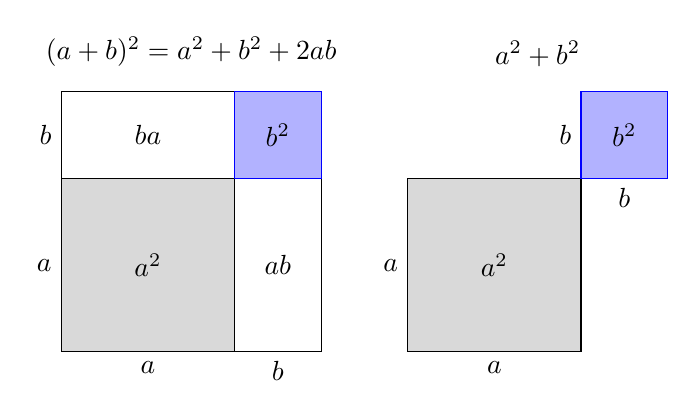
\begin{tikzpicture}[
node distance = 0pt,
gN/.style = {% gray Node
             draw, fill=gray!30, minimum size=22mm,
             inner sep=0pt, outer sep=0pt,
             node contents={$a^2$}},
bN/.style = {% blue Node
             draw=blue, fill=blue!30, minimum size=11mm,
             inner sep=0pt, outer sep=0pt,
             node contents={$b^2$}},
hN/.style = {draw, minimum height=11mm, minimum width=22mm,
             inner sep=0pt, outer sep=0pt,
             node contents={$ba$}},
vN/.style = {draw, minimum height=22mm, minimum width=11mm,
             inner sep=0pt, outer sep=0pt,
             node contents={$ab$}},
                        ]

\node (a)   [gN, label=left:$a$, label=below:$a$];
\node (ba)  [hN,above=of a, label=left:$b$];
\node (ab)  [vN,right=of a, label=below:$b$];
\node (b)   [bN,above=of ab];
\node[above=2mm of {$(ba.north west)!0.5!(b.north east)$}] {$(a+b)^2=a^2+b^2+2ab$};

\scoped[xshift=44mm]
{
\node (a)   [gN, label=left:$a$, label=below:$a$];
\node (b)   [bN,above right=of a, 
                label=left:$b$, label=below:$b$];
\node[above=2mm of {$(a.west |- b.north)!0.5!(b.north east)$}] {$a^2+b^2$};
}
    \end{tikzpicture}
\end{document}